\documentclass[11pt,a4paper]{article}
\usepackage[margin=23mm,headheight=16pt]{geometry}
\usepackage[T1]{fontenc}
\usepackage{tgpagella}
\usepackage{amsmath,amssymb,amsthm,mathtools,bm,microtype,booktabs,tabularx,enumitem}
\usepackage{tikz}
\usetikzlibrary{arrows.meta,positioning,calc,decorations.pathmorphing}
\usepackage{xcolor,fancyhdr,hyperref}
\definecolor{deepblue}{RGB}{25,50,99}
\definecolor{purple}{RGB}{104,69,170}
\definecolor{softblue}{RGB}{227,238,249}
\hypersetup{colorlinks=true,linkcolor=deepblue,urlcolor=deepblue}
\pagestyle{fancy}\fancyhf{}\fancyhead[L]{\small Quantum Entanglement and Optical Lattices}\fancyhead[R]{\small Quantum Physics Companion V}\fancyfoot[C]{\thepage}
\setlength{\parskip}{5pt}\setlength{\parindent}{0pt}
\setcounter{secnumdepth}{3}
\newtheorem{example}{Worked Example}
\newtheorem{remark}{Remark}
\newcommand{\tr}{\operatorname{Tr}}
\newcommand{\kb}{k_{\mathrm B}}
\begin{document}
\begin{center}
{\Large\bfseries\color{deepblue} Quantum Entanglement and Correlations\\ in Optical Lattices}\par\medskip
{\large Chapter V: Exact Many-Body States, Reduced Density Matrices,\\ Entropy, Correlation Functions and Measurement}\par\smallskip
{\small Detailed continuation of the Rubidium-87 and Bose--Hubbard Companion}\par
\end{center}
\begin{abstract}
This chapter distinguishes Bose--Einstein condensation, first-order coherence, number correlation and bipartite mode entanglement. It derives the exact two-boson/two-site ground state and reduced density matrix, diagonalizes the one-body density matrix, explains particle-number superselection, introduces spatial entanglement and mutual information, and sketches exact diagonalization on larger optical lattices. Every appearance of an ``orbital'' in the Bose--Hubbard theory means a Wannier orbital for a \emph{whole atom}, not the electronic $5s$ orbital of rubidium.
\end{abstract}
\tableofcontents
\clearpage
\section{What does a condensate wavefunction leave out?}
A dilute atomic condensate may be approximated by one macroscopic motional field $\Psi(\mathbf r)=\sqrt{n_0(\mathbf r)}e^{i\theta(\mathbf r)}$. This captures a density profile, phase gradients, and many mean-field observables. It does not, by itself, specify all higher-order many-body correlations. The precise many-body state is a vector in a Fock space of atomic modes, or a density operator for a mixed state.
We distinguish (i) \emph{condensation}, defined by macroscopic eigenvalue(s) of the one-body density matrix, (ii) \emph{first-order coherence}, encoded in $\langle a_i^\dagger a_j\rangle$, (iii) \emph{number correlations}, involving $\langle n_i n_j\rangle$, and (iv) \emph{entanglement}, which is defined only after specifying a partition into subsystems. These concepts are related but not interchangeable.
\begin{figure}[h!]
\centering
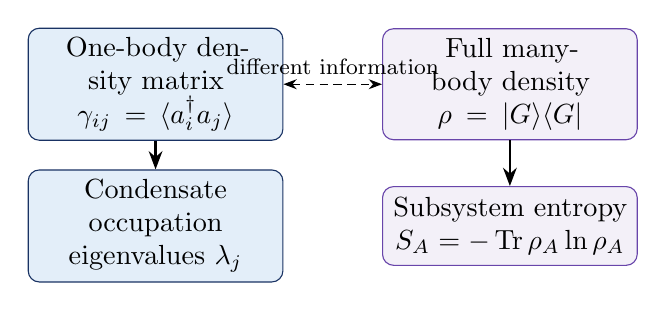
\begin{tikzpicture}[>=Stealth,scale=.9]
\node[draw=deepblue,rounded corners,fill=softblue,text width=3.0cm,align=center,minimum height=1cm] (a) at (0,0) {One-body density matrix\\$\gamma_{ij}=\langle a_i^\dagger a_j\rangle$};
\node[draw=purple,rounded corners,fill=purple!8,text width=3.0cm,align=center,minimum height=1cm] (b) at (5,0) {Full many-body density\\$\rho=|G\rangle\langle G|$};
\node[draw=deepblue,rounded corners,fill=softblue,text width=3cm,align=center,minimum height=1cm] (c) at (0,-2) {Condensate occupation\\eigenvalues $\lambda_j$};
\node[draw=purple,rounded corners,fill=purple!8,text width=3cm,align=center,minimum height=1cm] (d) at (5,-2) {Subsystem entropy\\$S_A=-\tr\rho_A\ln\rho_A$};
\draw[->,thick] (a)--(c);\draw[->,thick] (b)--(d);
\draw[<->,densely dashed] (a)--node[above,font=\footnotesize]{different information} (b);
\end{tikzpicture}
\caption{The one-body density matrix and the full many-body density operator answer different physical questions.}
\end{figure}
\section{Exact ground state of two bosons in a double well}
In the basis $\{|20\rangle,|11\rangle,|02\rangle\}$ the Bose--Hubbard Hamiltonian is
\begin{equation}H=\begin{pmatrix}U&-\sqrt2J&0\\-\sqrt2J&0&-\sqrt2J\\0&-\sqrt2J&U\end{pmatrix}.\end{equation}
Define $|S\rangle=(|20\rangle+|02\rangle)/\sqrt2$ and $|A\rangle=(|20\rangle-|02\rangle)/\sqrt2$. The antisymmetric state has energy $U$ and decouples. The symmetric block is
\begin{equation}H_{\rm sym}=\begin{pmatrix}U&-2J\\-2J&0\end{pmatrix}.\end{equation}
Its energies are $E_{\pm}=(U\pm D)/2$ where $D=\sqrt{U^2+16J^2}$. For $U\ge0$ and $J>0$, the ground state is
\begin{equation}\label{eq:ground}|G\rangle=A|S\rangle+B|11\rangle,\quad A=\sqrt{\frac{1-U/D}{2}},\quad B=\sqrt{\frac{1+U/D}{2}}.\end{equation}
Substituting this vector into $H_{\rm sym}|G\rangle=E_-|G\rangle$ verifies both the eigenvalue and normalization. A phase convention has been chosen so $A,B\ge0$.
\begin{example}[Noninteracting bosons share a bonding orbital]
For $U=0$, $A=B=1/\sqrt2$ and $|G\rangle=\tfrac12|20\rangle+2^{-1/2}|11\rangle+\tfrac12|02\rangle$. This equals $(b_+^\dagger)^2|0\rangle/\sqrt{2!}$ with $b_+^\dagger=(a_L^\dagger+a_R^\dagger)/\sqrt2$. There are still two whole atoms; both occupy one delocalized motional orbital.
\end{example}
\begin{example}[Strong repulsion and fixed occupation]
For $U/J\gg1$, $D\simeq U+8J^2/U$, so $A\simeq2J/U$ and $B\simeq1-2J^2/U^2$. Therefore $|G\rangle\simeq|11\rangle+(\sqrt2J/U)(|20\rangle+|02\rangle)$ to leading order. The Mott-like state contains small virtual double-occupancy amplitudes when $J\ne0$.
\end{example}
\section{Reduced density matrix and mode entanglement}
Write the state explicitly as $|G\rangle=(A/\sqrt2)|2\rangle_L|0\rangle_R+B|1\rangle_L|1\rangle_R+(A/\sqrt2)|0\rangle_L|2\rangle_R$. Tracing out the right subsystem gives, in the ordered left-site basis $\{|0\rangle,|1\rangle,|2\rangle\}$,
\begin{equation}\boxed{\rho_L=\tr_R|G\rangle\langle G|=\operatorname{diag}\left(\frac{A^2}{2},B^2,\frac{A^2}{2}\right).}\end{equation}
The purity and entropy are
\begin{align}\tr\rho_L^2&=B^4+\frac{A^4}{2},\\S_L&=-B^2\ln B^2-A^2\ln\left(\frac{A^2}{2}\right).\label{eq:entropy}\end{align}
Here logarithms are natural and the entropy is measured in nats. The entropy of a pure bipartite state is zero exactly when the state factorizes across the chosen left/right mode partition.
\begin{example}[Exact entropy at $U=0$]
Here $A^2=B^2=1/2$. Thus the eigenvalues of $\rho_L$ are $(1/4,1/2,1/4)$ and
\begin{equation}S_L=-\frac12\ln\frac12-2\frac14\ln\frac14=\frac32\ln2\approx1.03972.\end{equation}
The state is fully condensed in the bonding orbital but has nonzero left/right \emph{mode} entropy.
\end{example}
\begin{example}[Zero entanglement in the atomic Mott limit]
For $U/J\to\infty$, $A\to0$ and $B\to1$, hence $\rho_L\to|1\rangle\langle1|$, $\tr\rho_L^2\to1$, and $S_L\to0$. This is not evidence that all interacting lattice states are unentangled; it is the leading-order atomic-limit result for this particular partition and filling.
\end{example}
\begin{example}[Intermediate interaction $U/J=4$]
Then $D=4\sqrt2 J$, $B^2=(1+1/\sqrt2)/2\approx0.853553$ and $A^2\approx0.146447$. The reduced eigenvalues are approximately $(0.073223,0.853553,0.073223)$; substituting into Eq.~\eqref{eq:entropy} gives $S_L\approx0.518$ nats. This lies between the noninteracting and atomic-limit values.
\end{example}
\section{One-body density matrix and natural orbitals}
Define $\gamma_{ij}=\langle G|a_i^\dagger a_j|G\rangle$. For the symmetric ground state $\langle n_L\rangle=\langle n_R\rangle=1$. By Hellmann--Feynman,
\begin{equation}-\frac{\partial E_-}{\partial J}=\langle a_L^\dagger a_R+a_R^\dagger a_L\rangle=\frac{8J}{D}.\end{equation}
The off-diagonal expectation is real and equals $C=4J/D$, giving
\begin{equation}\boxed{\gamma=\begin{pmatrix}1&C\\C&1\end{pmatrix},\quad\lambda_\pm=1\pm C.}\end{equation}
The natural orbitals are the bonding and antibonding site combinations, $\phi_\pm=(\phi_L\pm\phi_R)/\sqrt2$. At $U=0$ the eigenvalues are $(2,0)$; as $U/J\to\infty$ they approach $(1,1)$. For a macroscopic system, condensation requires an eigenvalue that scales extensively with atom number; in this finite example the ratio $\lambda_+/N$ is simply a useful diagnostic, not proof of a thermodynamic phase.
\begin{example}[Condensation fraction versus mode entropy]
For $U/J=4$, $C=1/\sqrt2$, so $\lambda_+=1+1/\sqrt2\approx1.7071$ and $\lambda_-=1-1/\sqrt2\approx0.2929$. The largest-eigenvalue fraction is about $0.8536$, whereas $S_L\approx0.518$ nats. Neither number determines the other without knowledge of the many-body state.
\end{example}
\section{Number correlations and the particle-hole interpretation}
Since $n_L+n_R=2$, $\langle n_Ln_R\rangle=P_{11}=B^2$. For the connected covariance,
\begin{equation}\boxed{\operatorname{Cov}(n_L,n_R)=\langle n_Ln_R\rangle-\langle n_L\rangle\langle n_R\rangle=-A^2.}\end{equation}
Local occupation variance is $\operatorname{Var}(n_L)=A^2$. The equal-and-opposite relation follows from number conservation; it is not an independent signature of genuinely nonclassical entanglement. Classical mixtures with fixed total number can have nonzero negative number covariance.
\begin{example}[A classical mixture shares the same number probabilities]
Consider $\rho_{\rm mix}=(A^2/2)|20\rangle\langle20|+B^2|11\rangle\langle11|+(A^2/2)|02\rangle\langle02|$. It has the same occupation statistics and reduced diagonal density matrix as $|G\rangle$, but is separable across the mode bipartition and has no off-diagonal coherent superposition between these Fock configurations. Occupation histograms alone cannot establish entanglement.
\end{example}
\section{Important subtlety: identical particles and superselection}
For distinguishable qubits, tensor-product subsystems are naturally associated with particles. For identical bosons, the present partition is instead by \emph{spatial modes}, $\mathcal F_L\otimes\mathcal F_R$, in the occupation-number representation. Fixed total number gives local particle-number superselection restrictions. Consequently, the von Neumann mode entropy is a mathematically meaningful partition diagnostic, but the entanglement accessible under protocols that prohibit local number superpositions can differ from it. A fully delocalized single particle illustrates the issue: it has mode entropy $\ln2$, yet extracting a Bell pair with local operations under a strict particle-number superselection rule requires further resources. Thus an entanglement claim must specify modes, partitions, allowed operations and observables.
\section{Site mutual information and mixed states}
For a bipartite density matrix $\rho_{LR}$, define the mutual information
\begin{equation}I(L:R)=S(\rho_L)+S(\rho_R)-S(\rho_{LR}).\end{equation}
For a pure two-site state, $S(\rho_{LR})=0$ and symmetry implies $I(L:R)=2S_L$. For a mixed state, $I$ includes both quantum and classical correlations and is not itself an entanglement measure. At finite temperature, $\rho_T=e^{-\beta H}/Z$ must be used, and a nonzero $I$ does not prove entanglement.
\begin{example}[Pure-state mutual information]
At $U=0$, $I(L:R)=3\ln2\approx2.07944$ nats. As $U/J\to\infty$, $I\to0$. For a classically correlated 50--50 mixture of $|20\rangle$ and $|02\rangle$, the mutual information is nonzero even though the state is separable.
\end{example}
\section{Schmidt decomposition in the fixed-$N$ sector}
The expansion $|G\rangle=(A/\sqrt2)|2\rangle_L|0\rangle_R+B|1\rangle_L|1\rangle_R+(A/\sqrt2)|0\rangle_L|2\rangle_R$ is already a Schmidt decomposition up to ordering. Its Schmidt coefficients are $\{A/\sqrt2,B,A/\sqrt2\}$, and their squared moduli are the eigenvalues of $\rho_L$. The Schmidt rank is three for finite $J>0$ and two-boson repulsive $U$, collapsing to one in the strict $U/J\to\infty$ limit.
\begin{example}[Linear entropy as a simpler diagnostic]
The linear entropy is $S_{\rm lin}=1-\tr\rho_L^2=1-B^4-A^4/2$. At $U=0$, $S_{\rm lin}=1-(1/4+1/8)=5/8$. In the Mott limit it tends to zero. Unlike von Neumann entropy, it does not require logarithms.
\end{example}
\section{Generalizing to three and four sites}
For $N$ atoms on $L$ sites the fixed-number Fock-space dimension is $\binom{N+L-1}{L-1}$. For $N=L=3$ it is 10; for $N=L=4$ it is 35. Enumerate all $\mathbf n=(n_1,\ldots,n_L)$ with $\sum n_i=N$. The diagonal onsite energy is $\frac U2\sum_i n_i(n_i-1)$. A neighboring hop $j\to i$ carries amplitude $-J\sqrt{(n_i+1)n_j}$. Construct the sparse Hamiltonian, obtain its ground state numerically, and compute $\rho_A$ by grouping occupation configurations according to the chosen region $A$ and its complement. For example, a 4-site ring can be cut into two adjacent 2-site blocks; the entropy across that cut generally differs from single-site entropy.
\begin{figure}[h!]
\centering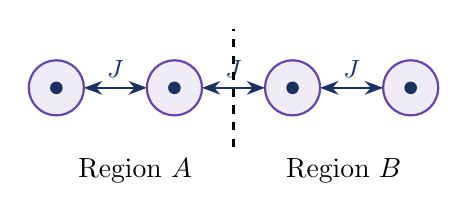
\begin{tikzpicture}[>=Stealth]
\foreach \x in {0,1.5,3,4.5} {\draw[purple,thick,fill=purple!10] (\x,0) circle(.35);\fill[deepblue] (\x,0) circle(.08);}
\foreach \x in {0.35,1.85,3.35} {\draw[<->,thick,deepblue] (\x,0)--++(.8,0) node[midway,above,font=\small] {$J$};}
\draw[dashed,thick] (2.25,-.75)--(2.25,.75);\node at (1,-1.05) {Region $A$};\node at (3.65,-1.05) {Region $B$};
\end{tikzpicture}\caption{A spatial bipartition of a four-site optical lattice. The bipartite entropy depends on the chosen cut.}
\end{figure}
\section{Why an entanglement area law is useful}
For many local gapped ground states, entanglement entropy scales primarily with the size of the boundary between regions rather than their full volume. In a one-dimensional chain, this can make tensor-network representations efficient, while near criticality logarithmic corrections and growing correlation lengths complicate approximations. A generic statement of an ``area law'' is not universal for every excited state, long-range Hamiltonian or critical dimension. The main research lesson is that spatial entanglement often determines whether matrix-product-state and density-matrix renormalization group methods can approximate an extended system well.
\section{Measurements: what can experiments actually infer?}
Time-of-flight interference probes one-body coherence; site-resolved microscopy yields number configurations and correlations; noise-correlation analysis accesses higher-order functions. Entanglement entropy is not simply read from one density image. Approaches include randomized measurements, interference between identical prepared copies, or model-assisted reconstruction; each requires explicit assumptions and experimental resources. For bosonic optical-lattice quantum simulators, quantum gas microscopy may measure site occupation and correlations, while direct entropy protocols are more demanding.
\begin{example}[Why interference visibility alone is insufficient]
The coherence $\langle a_L^\dagger a_R\rangle$ is zero for the pure Mott product $|11\rangle$, but it is also zero for many classically mixed density operators. Conversely, an interferometrically visible field need not have a large \emph{operationally accessible} bipartite entanglement under strict number superselection. Both a phase measurement and an entanglement certification protocol require a precise observable definition.
\end{example}
\section{Corrections, conventions and limitations}
Throughout, $J>0$ and $U\ge0$ unless stated. The system has two bosons and two modes; no sharp thermodynamic phase transition occurs. ``Site entanglement'' refers to a Fock-space mode tensor product, not individually labeled atomic particles. The $U\to\infty$ result is a limit at fixed $J>0$, while the $J=0$ atomic model has additional degeneracies in some particle-number sectors. An experimental rubidium sample may also contain finite-temperature excitations, multiple spin components, inhomogeneous trapping, loss, and higher-band occupations, none of which are included in the minimal model.
\section{Further problems, with guidance}
\begin{enumerate}[leftmargin=*,itemsep=4pt]
\item Derive the normalized exact two-site ground state, starting from the $2\times2$ symmetric Hamiltonian. \emph{Hint:} use the negative eigenvalue and normalize its eigenvector.
\item Show that the reduced state is diagonal in local particle number for any fixed-$N$ pure two-mode state. \emph{Hint:} the right mode occupation determines the left occupation.
\item Derive Eq.~\eqref{eq:entropy} and verify $S_L(U=0)=\tfrac32\ln2$.
\item Prove $\gamma=\begin{psmallmatrix}1&4J/D\\4J/D&1\end{psmallmatrix}$ by differentiating the ground-state energy.
\item Evaluate $P_{11}$, $\operatorname{Var}(n_L)$, the two natural-orbital occupations, and $S_L$ at $U/J=2$.
\item Demonstrate explicitly that $\rho_{\rm mix}$ and $|G\rangle\langle G|$ share number probabilities but differ in their coherence matrix elements.
\item Derive the linear entropy at arbitrary $U/J$ and its large-$U$ expansion.
\item Enumerate the 10 Fock states for $N=L=3$ and construct the open-chain hopping matrix.
\item Explain why a fixed particle-number condensate has $\langle a_j\rangle=0$ but may still show first-order coherence.
\item Compare mode entropy with operational entanglement under local number superselection, stating which operations are permitted.
\end{enumerate}
\section{Selected references}
\begin{enumerate}[leftmargin=*]
\item O. Penrose and L. Onsager, ``Bose--Einstein Condensation and Liquid Helium,'' \emph{Physical Review} 104 (1956), 576--584.
\item M. Greiner et al., ``Quantum phase transition from a superfluid to a Mott insulator in a gas of ultracold atoms,'' \emph{Nature} 415 (2002), 39--44.
\item I. Bloch, J. Dalibard and W. Zwerger, ``Many-body physics with ultracold gases,'' \emph{Reviews of Modern Physics} 80 (2008), 885--964.
\item L. Amico et al., ``Entanglement in many-body systems,'' \emph{Reviews of Modern Physics} 80 (2008), 517--576.
\item H. M. Wiseman and J. A. Vaccaro, ``Entanglement of Indistinguishable Particles Shared between Two Parties,'' \emph{Physical Review Letters} 91 (2003), 097902.
\item R. Horodecki et al., ``Quantum entanglement,'' \emph{Reviews of Modern Physics} 81 (2009), 865--942.
\end{enumerate}
\end{document}
